\subsubsection*{Exkurs: Differenz-Pipeline}

\begin{figure}[h!]
\centering
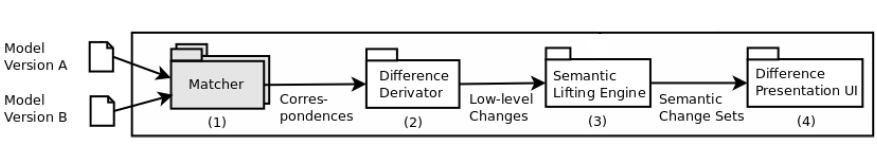
\includegraphics[width=\textwidth]{architecture/graphics/silift-pipeline.png}
\caption{SiLift Processing Pipeline}
\label{silift-pipeline}
\end{figure}

Die Vorgehensweise von SiLift lässt sich am besten mit einer vierstufigen \textit{Pipeline}, wie in Abbildung \ref{silift-pipeline} dargestellt,  vergleichen.
Als Eingabe dienen immer zwei Versionen eines Modells, z.B. \texttt{model\_A.ecore} und \texttt{model\_B.ecore} (Abb. \ref{classdiagram_example}):

\begin{enumerate}
\item \textbf{Matching}: Aufgabe eines \textit{Matcher} ist es die korrespondierenden Elemente aus Modell A und Modell B, also die Elemente, die in beiden Modellen übereinstimmen, zu identifizieren.
Dabei ist das Ergebnis vor allem davon abhängig anhand welcher Kriterien der Matcher eine Übereinstimmung festlegt.
Hier wird unter anderem unterschieden zwischen \textit{ID-}, \textit{signatur-} und \textit{ähnlichkeitsbasierten} Verfahren.\\
In SiLift stehen unter anderem folgende Matcher-Engines zur Verfügung:

\begin{itemize}
	\item \texttt{EcoreID Matcher}: Ein \textit{ID-basierter} Matcher (nutzt Werte von Attributen, die im Metamodell als ID-Attribute deklariert sind).
	\item \texttt{EMF Compare}: Unterstützt alle drei Verfahren. \texttt{EMF Compare} kann unter \texttt{Win\-dow} $\triangleright$ \texttt{Preferences}: \texttt{EMF Compare} konfiguriert werden. \footnote{Informationen zum \texttt{EMF Compare Project} finden Sie unter \url{http://www.eclipse.org/emf/compare}.}
	
	\item \texttt{NamedElement Matcher}: Ein signaturbasierter Matcher, welcher die ent\-sprech\-enden Korrespondenzen anhand der Werte der jeweiligen Namensattribute bestimmt.
	
	\item \texttt{URIFragment Matcher}: Ein signaturbasierter Matcher, welcher die ent\-sprech\-enden Korrespondenzen anhand der Werte der \textit{Uri} der Elemente bestimmt (z.B. \texttt{eType=}"'\texttt{ecore:EDataType http://www.eclipse.org/emf/2002/\-E\-core\-\#//EString}"').
	
	\item \texttt{UUID Matcher}: Ein ID-basierter Matcher. (basiert auf XMI-IDs der XMI-Repräsentationen der Modelle, falls vorhanden).
\end{itemize}
(Abb. \ref{silift-wizard_compare_page2}).
Diese Liste ist keineswegs abgeschlossen und kann durch zusätzliche Matching-Engines, wie z.B. \textit{SiDiff} oder auch eigener Matcher ergänzt werden.\footnote{Weitere Informationen zu \textit{SiDiff} finden Sie unter \url{http://pi.informatik.uni-siegen.de/Projekte/sidiff}}\\

\item \textbf{Difference derivation}: Ausgehend von den gefunden Korrespondenzen berechnet der \textit{Difference Derivator} eine technische Differenz (\textit{low-level difference}) der Mo\-del\-le.
Alle Objekte und Referenzen, für die keine Korrespondenz existiert müssen demnach entweder in Modell B hinzugefügt, oder aus Modell A entfernt worden sein (vgl. Abb. \ref{silift-technical_difference}).

\begin{figure}[h!]
\centering
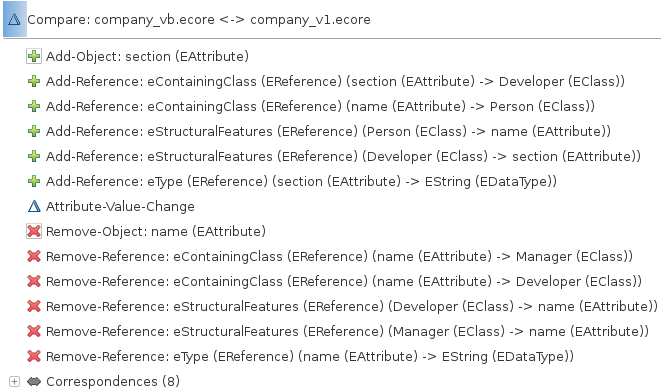
\includegraphics[width=0.8\textwidth]{architecture/graphics/silift-technical_difference.png}
\caption{technische Differenz von  \texttt{model\_vb.ecore} und \texttt{model\_v1.ecore}}
\label{silift-technical_difference}
\end{figure}

Die Berechnung der technischen Differen kann durch die Wahl des \textit{Technical Difference Builder} beeinflusst werden (vgl. Abb. \ref{silift-wizard_compare_page2}).

\item \textbf{Semantic Lifting}: Die zuvor berechnete technische Differenz enthält alle Änder\-ungen auf Basis des Metamodells.
Diese sollen nun \textit{semantisch geliftet} werden.
Dazu werden die einzelnen Änderungen mit Hilfe von \textit{Erkennungsregeln} (egnl. \textit{recognition rules}) in sogenannte \textit{Semantic Change Sets} gruppiert, die jeweils eine vom Benutzer ausgeführte \textit{Editieroperation} repräsentieren.
Mit der Wahl einer \textit{Rule Base} wird festgelegt, welche Erkennungsregeln zum liften benutzt werden sollen.
Dabei wird zwischen folgenden \textit{Rule Bases} unterschieden: \texttt{AtomicGenerated}, \texttt{Atomic\-Manual} und \texttt{Complex} (vgl. Abb. \ref{silift-wizard_compare_page1}).
Während atomare Regeln das Erzeugen, Löschen, Verschieben von Elementen und das Ändern der Attributwerte von Elementen umfassen, setzen sich die komplexen Editierregeln i.d.R. aus den atomaren und anderen komplexen Regeln zusammen.\footnote{Weitere Informationen zu den \textit{Recognition Rules} finden Sie im \textbf{SiLift - Benutzerhandbuch für Entwickler}.}
Welchen Einfluss die Wahl einer oder mehrerer \textit{Rule Bases} für das \textit{semantische Liften} hat wird später noch am Beispiel demonstriert.

\item \textbf{Difference Presentation UI}: \textit{SiLift} stellt einen \textit{Compare View} bereit, um Differenzen übersichtlich darzustellen.
\end{enumerate}

Damit endet die Pipeline.